% This is a default-selection of plugins that are used widely in this repo.

\documentclass[a4paper,10pt,fleqn]{article}
\usepackage[utf8]{inputenc}

% deutsche Trennmuster etc.
\usepackage[ngerman]{babel}
\usepackage[T1]{fontenc}

% mathematical simbols and fonts
\usepackage{mathtools} 
\usepackage{amssymb}
\usepackage{amsmath}
\usepackage{ntheorem}
\usepackage{polynom}
\usepackage{marvosym}
\usepackage{tabu}
\renewcommand*{\bmod}{\mathbin{\%}}
\everymath{\displaystyle}

\usepackage{multicol}
\usepackage{color}
\usepackage[usenames,dvipsnames]{xcolor}
\setlength{\columnsep}{1cm}
\setlength{\columnseprule}{0.25pt}
\def\columnseprulecolor{\color{gray}}
\usepackage{hyperref}

\usepackage[margin=1.5cm]{geometry}
\usepackage{graphicx}
\usepackage{pgfplots}
\pgfplotsset{compat=1.10}

%Code higlighting

\usepackage{minted}

% make lists more compact:
\newlength{\wideitemsep}
\setlength{\wideitemsep}{.5\itemsep}
\addtolength{\wideitemsep}{-5pt}
\let\olditem\item
\renewcommand{\item}{\setlength{\itemsep}{\wideitemsep}\olditem}
\renewcommand{\arraystretch}{1.25}

\title{Zusammenfassung Bsys2}
\author{Fabian Hauser}
 
\begin{document}
\maketitle
%\begin{multicols}{2}
%[
\section{Bsys2}
%]

\subsection{GUIs}


\subsection{Windows}
\subsubsection{Messages}

\begin{description}
	\item[Message-Loop] \hfill \\
		GetMessage()-Schlaufe, durch Events schleifen
	\item[PostMessage()] \hfill \\
		Message via Umgehung der Queue an den Window Thread senden
	\item[SendMessage()] \hfill \\
		Message via Umgehung der Queue an den Window Thread senden (blocking des versender-Threads (Deadlock möglich)
\end{description}

\subsubsection{Window}

Jede Window-Class hat einen Handler
Alle Events werden dem jeweilig Betroffenen Handler gemeldet.


\subsection{Unix / Linux}
\subsubsection{Protocol Stack}
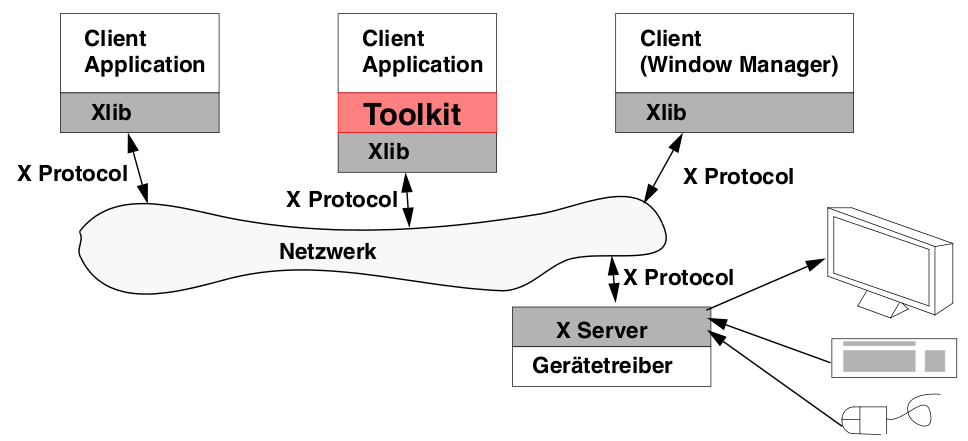
\includegraphics[width=\linewidth]{img/x_client_server.png}

\subsubsection{Client Reqests}
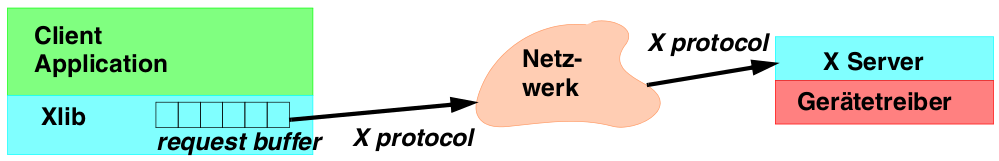
\includegraphics[width=\linewidth]{img/x_client_request.png}

\subsubsection{Server Events}
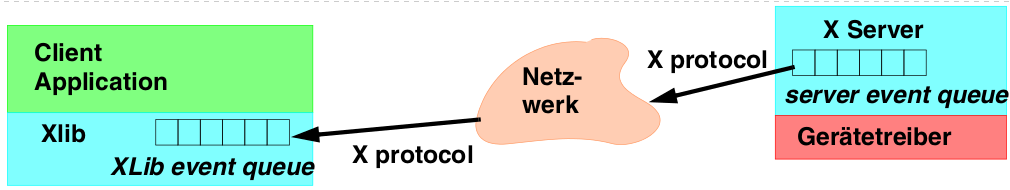
\includegraphics[width=\linewidth]{img/x_server_event.png}

%\end{multicols}
\end{document}